% ============================================================================
%  Problems: วงกลม (Circles)
%  Ordered from easy (basic) → intermediate.
%  Shared by exercise.tex and answer-key.tex
% ============================================================================

% --- Part 1: พื้นฐาน (Basic) ---
\examsection{ตอนที่ 1: พื้นฐาน — สูตรวงกลมและคอร์ด}

\problem{
  วงกลมมีรัศมี $7$ เซนติเมตร จงหาเส้นรอบวงและพื้นที่
  ($\pi \approx \frac{22}{7}$)
}{
  เส้นรอบวง $= 2\pi r = 2 \times \frac{22}{7} \times 7 = 44$ ซม.

  พื้นที่ $= \pi r^2 = \frac{22}{7} \times 49 = 154$ ตร.ซม.
}

\problem{
  วงกลมมีรัศมี $10$ ซม. และมุมที่จุดศูนย์กลาง $72^\circ$
  จงหาความยาวส่วนโค้งที่รองรับด้วยมุมนี้
}{
  $L = \dfrac{\theta}{360^\circ} \times 2\pi r
      = \dfrac{72}{360} \times 2\pi \times 10
      = \dfrac{1}{5} \times 20\pi = 4\pi$ ซม.
}

\problem{
  วงกลมมีรัศมี $6$ ซม. และมุมที่จุดศูนย์กลาง $120^\circ$
  จงหาพื้นที่เซกเตอร์ที่รองรับด้วยมุมนี้
}{
  $A = \dfrac{\theta}{360^\circ} \times \pi r^2
      = \dfrac{120}{360} \times \pi \times 36
      = \dfrac{1}{3} \times 36\pi = 12\pi$ ตร.ซม.
}

\problem{
  วงกลมมีรัศมี $5$ ซม. และมีคอร์ด $AB$ ยาว $8$ ซม.
  จงหาระยะห่างจากจุดศูนย์กลางถึงคอร์ด $AB$
}{
  ให้ $d$ = ระยะจากจุดศูนย์กลางถึงคอร์ด

  ครึ่งคอร์ด $= \frac{8}{2} = 4$ ซม.

  $d^2 + 4^2 = 5^2 \;\Rightarrow\; d^2 + 16 = 25 \;\Rightarrow\; d = 3$ ซม.
}

% --- Part 2: การประยุกต์ (Intermediate) ---
\examsection{ตอนที่ 2: การประยุกต์ — มุมในวงกลมและเส้นสัมผัส}

\problem{
  จากจุด $P$ ภายนอกวงกลม ลากเส้นสัมผัส $PA$ และ $PB$ ไปยังวงกลม
  โดย $PA = 12$ ซม. และระยะจาก $P$ ถึงจุดศูนย์กลาง $O$ เป็น $13$ ซม.
  จงหารัศมีของวงกลม
}{
  เส้นสัมผัสตั้งฉากกับรัศมี: $\triangle OAP$ เป็นสามเหลี่ยมมุมฉากที่ $A$

  $r^2 + 12^2 = 13^2 \;\Rightarrow\; r^2 + 144 = 169 \;\Rightarrow\; r = 5$ ซม.
}

\problem{
  ในวงกลมวงหนึ่ง มุมที่จุดศูนย์กลาง $\angle AOB = 120^\circ$
  จงหาขนาดของมุมในส่วนโค้ง $\angle ACB$ ที่รองรับด้วยส่วนโค้ง $AB$ เดียวกัน
}{
  มุมในส่วนโค้ง $= \dfrac{1}{2} \times$ มุมที่จุดศูนย์กลาง

  $\angle ACB = \dfrac{1}{2} \times 120^\circ = 60^\circ$
}

\problem{
  $AB$ เป็นเส้นผ่านศูนย์กลางของวงกลม และ $C$ เป็นจุดใด ๆ บนเส้นรอบวง
  จงหาขนาดของ $\angle ACB$
}{
  มุมในครึ่งวงกลมเป็นมุมฉากเสมอ

  $\angle ACB = 90^\circ$
}

\problem{
  $A$, $B$, $C$, $D$ เป็นจุดบนเส้นรอบวงของวงกลมเดียวกัน
  โดย $C$ และ $D$ อยู่บนส่วนโค้งเดียวกันของคอร์ด $AB$
  ถ้า $\angle ACB = 35^\circ$ จงหา $\angle ADB$
}{
  มุมในส่วนโค้งเดียวกันมีขนาดเท่ากัน

  $\angle ADB = 35^\circ$
}

\problem{
  รูปสี่เหลี่ยม $ABCD$ แนบในวงกลม
  ถ้า $\angle A = 85^\circ$ และ $\angle B = 70^\circ$
  จงหาขนาดของ $\angle C$ และ $\angle D$
}{
  มุมตรงข้ามรวมกัน $= 180^\circ$

  $\angle C = 180^\circ - 85^\circ = 95^\circ$

  $\angle D = 180^\circ - 70^\circ = 110^\circ$
}

\problem{
  เส้นตรง $PT$ สัมผัสวงกลมที่จุด $T$ และคอร์ด $TQ$ ลากจากจุด $T$
  ถ้ามุมระหว่างเส้นสัมผัส $PT$ กับคอร์ด $TQ$ เป็น $42^\circ$
  จงหาขนาดของมุมในส่วนโค้งตรงข้าม (alternate segment)
}{
  มุมระหว่างเส้นสัมผัสกับคอร์ด = มุมในส่วนโค้งตรงข้าม

  มุมในส่วนโค้งตรงข้าม $= 42^\circ$
}

% --- Part 3: ระดับ สอวน. (POSN Level) ---
\examsection{ตอนที่ 3: ระดับข้อสอบ สอวน.}

\problem{
  (ข้อสอบจริงปี 68 ข้อ 28) บริษัทแห่งหนึ่งต้องการขนส่งนํ้ามันโดยใช้ถังเหล็กทรงกระบอกขนาดใหญ่ ซึ่งแต่ละถังมีเส้นผ่านศูนย์กลาง 2 ฟุต เพื่อความปลอดภัยในการขนส่ง วิศวกรจึงจะจัดเรียงถังจำนวน 3 ใบ ให้อยู่ในลักษณะสัมผัสกันเป็นรูปสามเหลี่ยมดังรูป จากนั้นใช้สายเหล็กพันรอบถังทั้งสามใบ เพื่อให้ถังคงรูปและไม่กลิ้งออกจากกันในระหว่างการเคลื่อนย้าย   
จงหาว่า ความยาวของสายเหล็กสั้นที่สุด (หน่วยเป็นฟุต) ที่สามารถพันรอบถังทั้งสามใบนี้ได้อย่างพอดีใน 1 รอบ 
  \begin{center}
    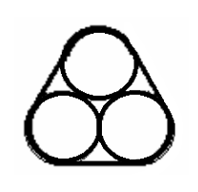
\includegraphics[width=0.2\textwidth]{images/geometry-circles-01.png}
  \end{center}
}{
  $6+2\pi$
}

\problem{
  (ข้อสอบจริงปี 65 ข้อ 12) ให้วงกลมรัศมี 5 หน่วย ถ้ามีคอร์ดยาว 5 หน่วยตัดวงกลมออกเป็นสองส่วน แล้วพื้นที่ของส่วนใหญ่มีค่าเท่ากับเท่าใด
}{
  $\dfrac{250\pi+75\sqrt{3}}{12}$
}